%!TEX root = ../template.tex
%%%%%%%%%%%%%%%%%%%%%%%%%%%%%%%%%%%%%%%%%%%%%%%%%%%%%%%%%%%%%%%%%%%
%% chapter1.tex
%% NOVA thesis document file
%%
%% Chapter with introduciton
%%%%%%%%%%%%%%%%%%%%%%%%%%%%%%%%%%%%%%%%%%%%%%%%%%%%%%%%%%%%%%%%%%%
\chapter{Experimental Observations and Validations}
\label{cha:experimentalEvaluation}

In this chapter we describe the work we conducted for the validation and evaluation of our proposed solution. 

We start by presenting the metrics we intend to evaluate, along with the test benchs we defined to test our prototype.
We then go deeper about each test bench, describing the results obtained during the experimental evaluation of each one of those scenarios, leading to a discussion later in this chapter aiming to compare those results and, finally, ending with a summary of the chapter.


\section{Criteria for Experimental Observations}
\label{sec:criteriaForExperimentalObservations}

Our evaluation process is simple: to track our TREDIS solution's behavior through all the different configurations, incrementally adding more layers to the system. Thus, we intend to evaluate our TREDIS solution on each possible configuration, starting with a basic model and slowly add more components to the system, while also making experimental observations about the impact they have. 

During the evaluation process we focused on measuring: 1) the performance impact each component has in the system while running with or without \gls{sgx}, through latency and throughput analysis, and 2) resource allocation during runtime, including memory and CPU usage. 

There are other particular measurements that we found useful to introduce, that we detailed later, while describing the test benchs individually.
Adding to that, we also analysed the system's behavior under different client-workloads, by scaling the number of requests and varying the typology of requests made over the system.


\section{Deployment Of Testbench Environments}
\label{sec:testBenchEnvironments}

As said before, we intend to evaluate our in-memory TREDIS system behavior by incrementally adding components to it, which will add security to the whole system, and see what impact they have on it. In order to do that, we defined a list of Test Benches (TB) that helped us evaluate the system. 

First, our idea was to benchmark a Single Redis instance, running normally inside our cloud server, to use it as a reference point to what is the regular behavior of a Redis \gls{kvs} in a system. Thus, we defined the TestBench 1 (TB1) as a Single instance Redis alone, with TLS support.

As the next step, we analyzed the impact \gls{sgx} has in a \gls{sgx}-enabled Redis instance. For that we defined TB2 as a Single instance Redis with TLS support running inside a SGX-enabled SCONE container, and benchmarked it.

TB3 includes the addition of the Proxy component, in order to benchmark its impact on the system. Thus, we defined TB3 as a Single instance Redis with TLS support running inside a SGX-enabled SCONE container, along with a Single Proxy instance.

In TB4, we placed the Proxy component on top of \gls{sgx}, resulting on benchmarking a system composed by a Single instance Redis with TLS support running inside a SGX-enabled SCONE container, along with a Single Proxy instance running inside \gls{sgx}.

For TB5, we added the attestation property to the components, used to assure that they indeed run in private memory regions on top of \gls{sgx} and by the correct defined enclave itself. Here we measure the impact it has to attestate each component upon start.

After that, with all the system model defined in \ref{cha:systemModel_and_design} in place, we created two more test benches TB6 and TB7 to evaluate the whole system behavior against different client request overloads (10k requests vs 100k requests) and against different typologies of requests (i.e., 10\% Writes:90\% Reads), respectively.

We proceeded the evaluation by performing these seven test bench evaluations over a system configured to run with the remaining two Redis \gls{kvs} configurations, Master-Slave and Cluster.


\section{Observations with Cloud-based Single REDIS}
\label{sec:cloudS_Redis}

In this section, we analize our solution running the in-memory Redis component configured as a Single instance \gls{kvs}. The experimental evaluation will be done following the test benches defined above, in order to study the impact of \gls{sgx} in our system, analysing both the performance and resource allocation impact that each secured component has in the system.

As we detailed in \ref{sec:implementationArchitecture}, we run our solution on a cloud system with \gls{sgx}-enabled hardware, while our client benchmark applications run on a local machine with commodity hardware, in order to simulate a real-world use-case where the network has a major impact in the performance of a system.

\subsection{Latency Impact of SGX-Enabled REDIS}

To study and compare the latency levels of our solution with and without \gls{sgx}, we evaluated our solution by complying to the test benches TB1, TB2, TB3 and TB4 (see \ref{sec:testBenchEnvironments} for details) definitions, with network conditions of ~116Mb/s Download and ~114Mb/s Upload speed. It is important to mention that, for the first two test benches where our client applications point directly to the Redis \gls{kvs} layer, we used redis-benchmark to make the requests and benchmark the solution. However, with the addition of the Proxy layer in TB3, we had to switch to a HTTP-enabled client - Jmeter.

Comparing the latency difference between TB1 and TB2, we observed that the addition of \gls{sgx} security properties to the \gls{kvs} component induced a latency overhead of 4,89\%, as we can see at Table  \ref{table:latencySingleRedis}.

%\begin{figure}[htbp]
%	\centering
%	{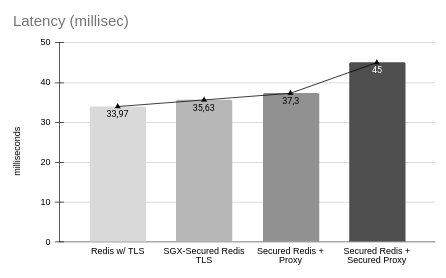
\includegraphics[width=0.8\linewidth]{graphLatency1234}}
%	\caption{Latency impact of SGX on single instance TREDIS}
%	\label{fig:graphLatencyStandalone}
%\end{figure}

\begin{table}[ht]
	\caption{Latency impact of SGX in Standalone Redis} % title of Table
	\centering % used for centering table
	\begin{tabular}{c c} % centered columns (4 columns)
		\hline\hline %inserts double horizontal lines
		\textbf{Configuration} & \textbf{Latency} \\ [0.5ex] % inserts table
		%heading
		\hline
		Redis & 33,97ms\\
		\hline
		SGX-enabled Redis & 35,63ms \\
		\hline
	    SGX-enabled Redis + Proxy & 37,3ms \\
		\hline % inserts single horizontal line
	    SGX-enabled Redis + SGX-enabled Proxy & 44ms\\ [1ex] % [1ex] adds vertical space
		\hline %inserts single line
	\end{tabular}
	\label{table:latencySingleRedis} % is used to refer this table in the text
\end{table}

However, as we detailed before in previous chapters, our TREDIS solution includes also a Proxy component that also adds overhead to the system, specially when also running inside \gls{sgx}. For that analysis, we run TB3 and TB4, in order to evaluate Proxy's impact in the overall system. Thus, with the addition of the Proxy, we observed an additional 4,69\% overhead compared with TB2, that we consider to be worth due to the purpose we give to this component. However, the 17,96\% latency increase that \gls{sgx} imposes to the Proxy component can lead to a subjective conclusion, depending on how important it is for the system to secure this entry point.

\subsection{Generic Throughput Observation}

In order to measure the impact that enabling \gls{sgx} has on the throughput of the solution, we followed the same test benches as the ones used before - TB1, TB2, TB3 and TB4. Our following evaluation is based on the average measurements of a few identical tests, each one consisting on one client (thread) making 10 000 requests with 3 Bytes length over the network.

\begin{figure}[htbp]
	\centering
	{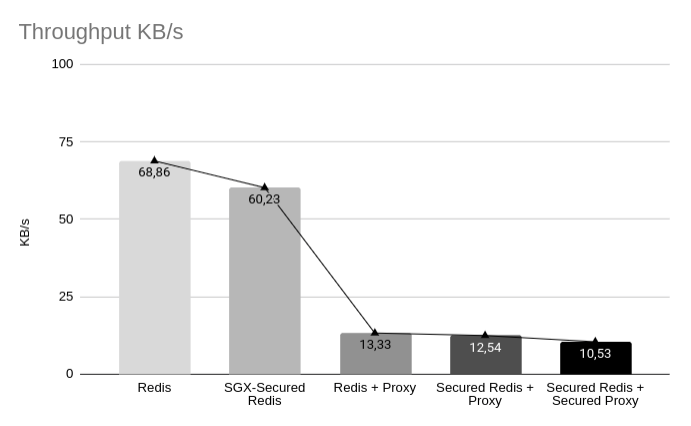
\includegraphics[width=0.8\linewidth]{graphThroughputStandalone}}
	\caption{SGX throughput impact - Standalone TREDIS}
	\label{fig:graphThroughputStandalone}
\end{figure}

Here, the addition of \gls{sgx} to the Redis component induced in a 28,71\% overhead, that can be observed in Figure \ref{fig:graphThroughputStandalone} in the tests made via redis-benchmark, in which the client application connects directly with the \gls{kvs} layer itself, via TCP requests. 

However, in TB3 and TB4, we can see that adding the Proxy component to the system dropped significantly the solution's throughput levels. This is expected since it allowed the requests to be done via HTTP, which induces an extra layer of overhead compared to TCP. With the requests being done via HTTP to the Proxy, we observed only a 5,93\% throughput penalty on running the \gls{kvs} on top of \gls{sgx}, which can be seen in Table \ref{table:throughputSingleRedis}, along with a 16,02\% drop when enabling the Proxy layer to also execute on top of \gls{sgx}.


\begin{table}[ht]
	\caption{Throughput impact of SGX} % title of Table
	\centering % used for centering table
	\begin{tabular}{c c} % centered columns (4 columns)
		\hline\hline %inserts double horizontal lines
		\textbf{Configuration} & \textbf{Throughput} \\ [0.5ex] % inserts table
		%heading
		\hline
		Redis + Proxy & 13,33KB/s\\
		\hline
		SGX-enabled Redis + Proxy & 12,54KB/s \\
		\hline % inserts single horizontal line
		SGX-enabled Redis + SGX-enabled Proxy & 10,53KB/s\\ [1ex] % [1ex] adds vertical space
		\hline %inserts single line
	\end{tabular}
	\label{table:throughputSingleRedis} % is used to refer this table in the text
\end{table}

(TODO TODO TODO) - Attestation

\subsection{Evaluation of Specific Benchmarks and Operations}

As a way to evaluate our solution's behavior facing more specific benchmarks, we tested the service by following the TB6 and TB7. 

Here we studied how different operation ratios influence the system throughput. By looking at Figure \ref{fig:thptDiffCombinationsSingleRedis}, we can see that there is not a big difference on how TREDIS handles these different combinations of requests with small payloads, by looking at the Total values, which remain relatively stable, showing only a slight throughput advantage when there is a majority of Writes in the database.

\begin{figure}[htbp]
	\centering
	{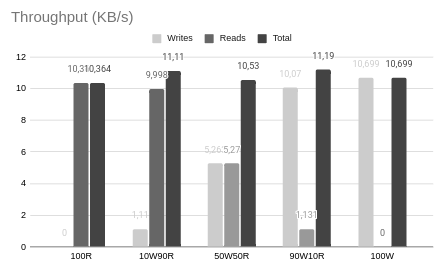
\includegraphics[width=0.8\linewidth]{thptDiffCombinationsSingleRedis}}
	\caption{SGX throughput impact - Standalone TREDIS}
	\label{fig:thptDiffCombinationsSingleRedis}
\end{figure}

However, as we increase the payload of the requests, we start to see a bigger difference in the throughput of the requests in favor of the Read operations, as we can see in the Table \ref{table:throughputPayloads}.

\begin{table}[ht]
	\caption{Throughput differences with different sized payloads} % title of Table
	\centering % used for centering table
	\begin{tabular}{c c c} % centered columns (4 columns)
		\hline\hline %inserts double horizontal lines
		\textbf{Payload Size} & \textbf{Read} & \textbf{Write} \\ [0.5ex] % inserts table
		%heading
		\hline
		3B & 10,364KB/s & 10,699KB/s\\
		\hline
		10KB & 208,33KB/s & 9,43KB/s \\
		\hline % inserts single horizontal line
		100KB & 1507,23KB/s & 5,31KB/s\\ [1ex] % [1ex] adds vertical space
		\hline %inserts single line
	\end{tabular}
	\label{table:throughputPayloads} % is used to refer this table in the text
\end{table} 

Also, to comply with TB6, we scaled the number of requests made to the server, in order to see differences in the behavior of the system. However, we found it hard to simulate \gls{epc} memory page swapping with small payloads, as it takes a long time to reach near the \gls{epc} memory size, so we incremented the size of the requests to 500KB. By doing that, we encountered an unexpected problem: when reaching the max heap size defined for Redis upon start, the container stopped working. We later found out that this problem is targeted in SCONE's website\footnote{https://sconedocs.github.io/faq/}, where it is explained this happens due to the SGX version (SGX v1) we are using not supporting dynamic allocation of memory, thus \textit{"enclaves must allocate all memory at startup since enclaves are fixed"}. This causes the memory usage of Redis to be higher than it needs to be, since to prevent it from crashing, we need to allocate memory upon start that we don't know we will need, which leads to larger startup times. However, SCONE also affirms that the next version of SGX (SGX v2) will support dynamic allocation, which tackles this problem. 

Thus, in order to test the EPC swap impact in the system, we (TODO TODO TODO)


\subsection{S-REDIS and Cloud System Resources}

Tabela:

running 100k benchmark: CPU 2\%

-	Cloud:    memory,  CPU Workoad, ..    
( tools para calcular po sistema em si : ps,   mmap,    ...)  
( tools para calcular po servidor Redis ( redis console ...))

\section{Observations with Cloud-based Master-Slave REDIS}
\label{sec:cloud_MS_Redis}

Here we present what we observed while testing our solution running Redis in a Master-Slave configuration. The experimental evaluation will be done following the same test benches that we used in Section \ref{sec:cloudS_Redis}, to analyze the impact that enabling \gls{sgx} support to our components have in the whole solution.

As we detailed in \ref{sec:implementationArchitecture}, we run our solution on a cloud system with \gls{sgx}-enabled hardware, while our client benchmark applications run on a local machine with commodity hardware, in order to simulate a real-world use-case where the network has a major impact in the performance of a system.


\subsection{Latency and impact of SGX-Enabled Master-Slave REDIS}

\begin{table}[ht]
	\caption{Latency impact of SGX in Standalone Redis} % title of Table
	\centering % used for centering table
	\begin{tabular}{c c} % centered columns (4 columns)
		\hline\hline %inserts double horizontal lines
		\textbf{Configuration} & \textbf{Latency} \\ [0.5ex] % inserts table
		%heading
		\hline
		Redis & 32,48ms\\
		\hline
		SGX-enabled Redis & 32,97ms \\
		\hline
		SGX-enabled Redis + Proxy & 34,45ms \\
		\hline % inserts single horizontal line
		SGX-enabled Redis + SGX-enabled Proxy & 41ms\\ [1ex] % [1ex] adds vertical space
		\hline %inserts single line
	\end{tabular}
	\label{table:latencyMasterSlaveRedis} % is used to refer this table in the text
\end{table}

\subsection{Generic throughput comparative observations}
// Single Instance vs. M/S

\begin{figure}[htbp]
	\centering
	{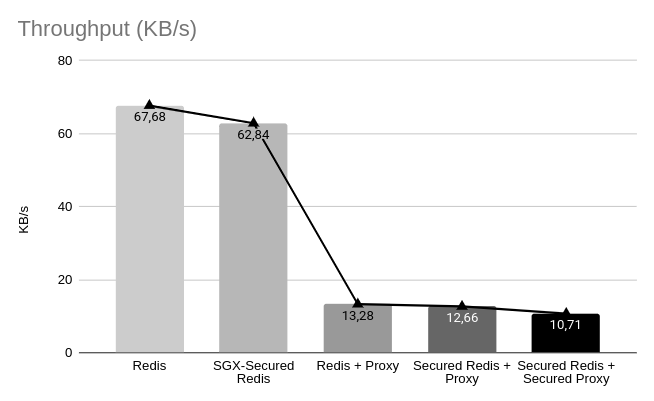
\includegraphics[width=0.8\linewidth]{graphThroughputMasterSlave}}
	\caption{SGX impact in MasterSlave}
	\label{fig:graphTroughputMasterSlave}
\end{figure}

\begin{table}[ht]
	\caption{Throughput impact of SGX} % title of Table
	\centering % used for centering table
	\begin{tabular}{c c} % centered columns (4 columns)
		\hline\hline %inserts double horizontal lines
		\textbf{Configuration} & \textbf{Throughput} \\ [0.5ex] % inserts table
		%heading
		\hline
		Redis + Proxy & 13,28KB/s\\
		\hline
		SGX-enabled Redis + Proxy & 12,667KB/s \\
		\hline % inserts single horizontal line
		SGX-enabled Redis + SGX-enabled Proxy & 10,71KB/s\\ [1ex] % [1ex] adds vertical space
		\hline %inserts single line
	\end{tabular}
	\label{table:throughputMasterSlaveRedis} % is used to refer this table in the text
\end{table}

\subsection{Throughput with benchmarks and specific operations}

text to get the graph to go down

\begin{figure}[htbp]
	\centering
	{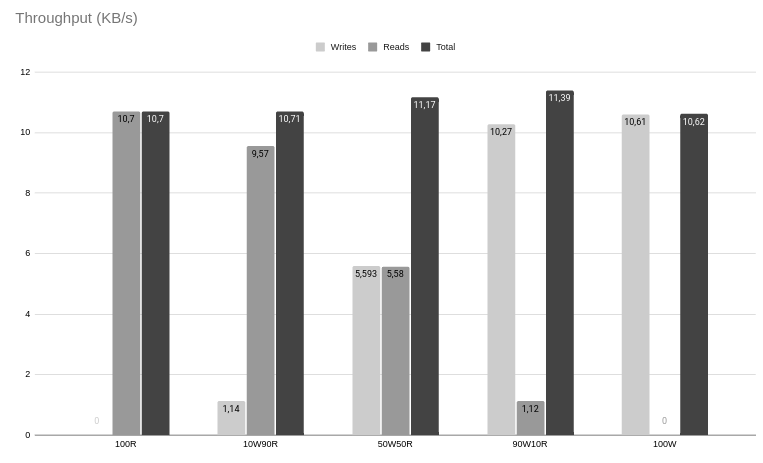
\includegraphics[width=0.8\linewidth]{thptDiffCombinationsMasterSlaveRedis}}
	\caption{SGX impact in MasterSlave}
	\label{fig:thptDiffCombinationsMasterSlaveRedis}
\end{figure}

\subsection{M/S REDIS and Cloud system resources}

P 59mb	RM 37mb	 RS1 37mb  RS2 37mb

Memory usage doesnt change with the test we made 5k reqs of 10kb payload, same results

\begin{figure}[htbp]
	\centering
	{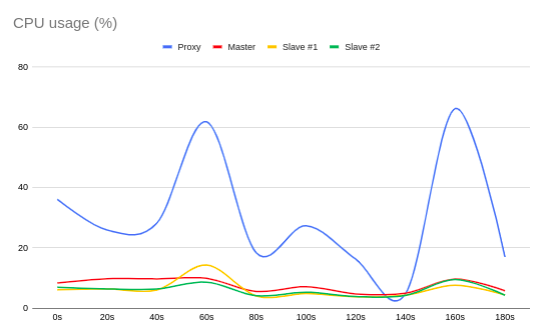
\includegraphics[width=0.8\linewidth]{cpuUsageMasterSlave}}
	\caption{SGX impact in MasterSlave}
	\label{fig:cpuUsageMasterSlave}
\end{figure}

\section{Observations with Cloud-based Clustered REDIS}
Mm cena mas po cluster

\subsection{Latency and impact of SGX-enabled REDIS Cluster}

\subsection{Comparative throughput: S  vs. M/S vs. CLUSTERED Redis}

\subsection{Clustered REDIS and Cloud System resources}

\section{Main findings from the experimental observations}

Comparar o 5.3, 5.4 e 5.5

\section{Sumamry}


